\section{Podklasy języków bezkontekstowych}
\label{cfl-subclassses}

\subsection{Definicje}

\begin{definition}  
    Gramatyka jest \textbf{liniowa} wtedy i tylko wtedy, gdy po prawej stronie każdej produkcji znajduje się maksymalnie jeden nieterminal.
\end{definition}

\begin{definition}
    Język \(L \subset \Sigma^*\) należy do klasy języków \textbf{\textsc{LinCFL}} (linear context-free language; LCFL) jeśli istnieje taka \textsc{LinCFG} \(A\), że \(L(A) = L\).
\end{definition}

\begin{definition}
    Definiujemy \textbf{deterministyczny automat ze stosem} (DPDA - deterministic pushdown automaton) tak jak zwykłe PDA, przy czym:
    
    \begin{itemize}
        \item Dla każdych \( a \in \Sigma, q \in Q, b \in \Gamma \), jeśli \( \delta(q, \eps, b) \not = \varnothing \) to \( \delta(q, a, b) = \varnothing \) (to znaczy, jeśli z jakiegoś stanu możemy wykonać \(\eps\)-przejście przy danym symbolu na szczycie stosu, to nie możemy w takiej sytuacji zrobić niczego innego).
        \item Dla każdych \( q \in Q, a \in (\Sigma \cup \eps) , b \in \Gamma \) jest tak, że \( |\delta(q, a, b)| = 1\), to znaczy jeśli mamy zdefiniowane przejście w jakiejś sytuacji to jest ono jednoznacznie określone. 
    \end{itemize}
\end{definition}

\begin{definition}
    Język \(L \subset \Sigma^*\) należy do klasy języków \textbf{DCFL} (deterministic contex-free langauage) jeśli istnieje taki DPDA \(A\), że \(L(A) = L\).
\end{definition}

\subsection{Zawierania}

Aby być w stanie sensownie dowodzić, że nie ma pewnych zawierań między różnymi podklasami języków bezkontekstowych musimy wprowadzić lemat o pompowaniu dla języków generowanych przez gramatyki liniowe (czyli języków należących do klasy \textsc{LinCFL}).

\begin{theorem}[O pompowaniu dla języków liniowych]
    \large
    \[ 
    \begin{split}
        &\forall_{L \in \textsc{LinCFL}}  \\
        &\exists_{n \in \natural} \\
        &\forall_{w \in L : |w| \geq n} \\
        &\exists_{uvpxy = w} |uvxy| \leq n \land |vx| \geq 1 \\
        &\forall_{i \in \natural} uv^ipx^iy \in L
    \end{split}
     \]
        
\end{theorem}

Czyli dzielimy słowo na pięć częsci, wszystkie poza środkową wchodzą do długości, a pompujemy drugą i czwartą.

\begin{proof}
    Bierzemy \(n = 4 \cdot |N| \cdot k \), gdzie jako \(k\) oznaczamy długość najdłuższej formy zdaniowej po prawej stronie wszystkich wywodów w gramatyce. W wywodzie generującym każde słowo takiej długości musi pojawić się jakiś nieterminal A, taki że:
    
    \[ 
        S \rightarrow_{G}^{k_0}\alpha A \beta \rightarrow_{G}^{k_1} \alpha \gamma A \delta \beta 
    \]
    
    gdzie \(k_1, k_2 \in \natural\), \(\alpha, \beta, \gamma, \delta \in \Sigma^* \), a \(A \in N\). 
    
    Zauważam, że jako że w wywodzie dopóki są nieterminale to jest dokładnie jeden (bo to jest gramatyka liniowa) to od razu wiem, że \( A \rightarrow_G^{k_1} \gamma A \delta \) dla \( \gamma, \delta \in \Sigma^* \). W takim razie mogę ,,podstawiać'' coś takiego za \(A\) tyle razy ile chcę (w szczególności mogę w ogóle pominąć tę ,,pętlę'') skąd mam, że: 
    
    \[
        \forall_{i \in \natural} S \rightarrow_{G}^* \alpha \gamma^i A \delta^i \beta 
    \]

    Jednocześnie, \(A\) ma w domknięciu przechodnim jakieś słowo (bo inaczej nie pojawiłoby się w wywodzie dla słowa \(w\)). Reasumując, \( \exists_{x \in \Sigma^*} A \rightarrow_G^* x \), a stąd już mamy, że: 
    
    \[ 
        \forall_{i \in \natural} S \rightarrow_{G}^* \alpha \gamma^i x \delta^i \beta 
    \] 
    
    dla pewnych \( \alpha, \beta, \gamma, \delta, x \in \Sigma^* \). 
    
    Wiemy, że \( |\gamma\delta| \geq 1 \), bo inaczej słowo byłoby za krótkie - powtórzenie przecież powstało, żeby słowo było właśnie odpowiednio długie.
    
    Jednocześnie \( |\alpha\gamma\delta\beta| \leq n\), bo zanim doszło do powtórzenia to nie mogliśmy ,,wypisać'' więcej liter niż długość maksymalnej strony wywodu przemnożona przez liczbę nieterminali.
    
\end{proof}

Dla rozjaśnienia sytuacji, rysunek poglądowy:

\begin{center}
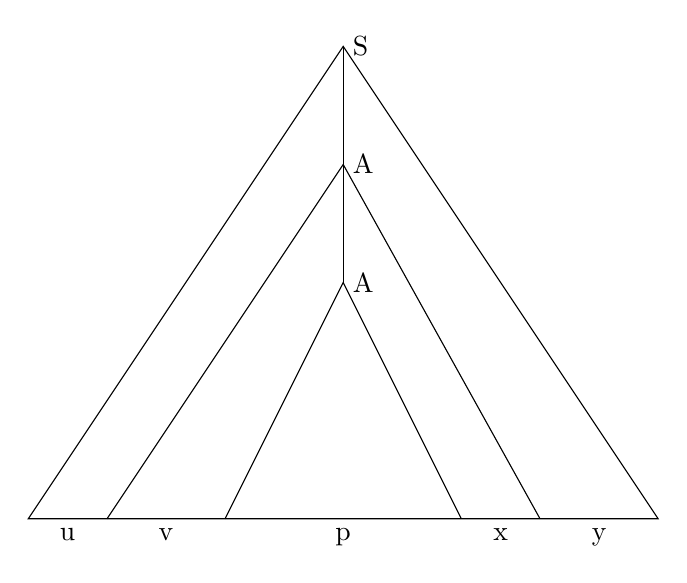
\begin{tikzpicture}
    \draw (4,0) -- (0,-6) -- (8,-6) -- cycle;
    \draw (4,0) -- (4,-1.5) -- (4, -3);
    \draw (1,-6) -- (4,-1.5) -- (6.5,-6);
    \draw (2.5,-6) -- (4,-3) -- (5.5,-6);

    \node[right] at (4,0) {S};
    \node[right] at (4,-1.5) {A};
    \node[right] at (4,-3) {A};
    \node[below] at (0.5,-6) {u};
    \node[below] at (1.75,-6) {v};
    \node[below] at (4,-6) {p};
    \node[below] at (6,-6) {x};
    \node[below] at (7.25,-6) {y};
\end{tikzpicture}
\end{center}

Widać, że możemy dodawać (lub usunąć) cykle \(A \rightarrow A\) które to generują nam \(v, x\) w odpowiednim miejscu.

Uzbrojeni w to twierdzenie oraz pamiętając poprzednie, możemy udowodnić odpowiednie nierówności zawierania:

\begin{theorem}
    \(\textsc{LinCFL} \not \subset \reg{\Sigma} \) oraz \(\textsc{DCFL} \not \subset \reg{\Sigma}\)
\end{theorem}

\begin{proof}
    Język \( \set{a^nb^n : n\in \natural} \) istnieje. Możemy skonstruować prostą gramatykę i proste DPDA które go rozpoznaje, ale wiemy (z lematu o pompowaniu dla wyrażeń regularnych) że język ten nie jest regularny.
\end{proof}

\begin{theorem}
    \( \reg{\Sigma} \subset \textsc{LinCFL} \) oraz \( \reg{\Sigma} \subset \textsc{DCFL}\)
\end{theorem}

\begin{proof}
    W pierwszym przypadku dosyć prosto skonstruować gramatykę liniową, która oddaje swoimi przejściami operacje które można robić na regexach, w drugim przypadku konwersja DFA na DPDA jest trywialna.
\end{proof}

Teraz pora na ciekawsze zawierania (a raczej braki tychże). 

\begin{theorem}
    \( \textsc{DCFL} \not \subset \textsc{LinCFL} \)
\end{theorem}

\begin{proof}
    Rozpatrzmy język \(L_{BAL}\) (ten ze zbalansowanymi nawiasowaniami). Na pewno jest on w DCFL, ale z lematu o pompowaniu dla bezkontekstowych języków liniowych się on wywali (wystarczy spróbować zdepompować słowo postaci \( (^n)^n(^n)^n \), gdzie \(n\) to stała z lematu o pompowaniu).
\end{proof}

\begin{theorem}
     \( \textsc{LinCFL} \not \subset \textsc{DCFL} \)
\end{theorem}
\begin{proof}
    Zbiór \(\braces{a^nb^n: n \in \natural} \cup \braces{a^nb^{2n}:n\in\natural}\) jest \textsc{LinCFL},
    ale deterministyczny automat ze stosem ma tylko jedną ścieżkę obliczeń, więc po dojściu do pierwszego stanu akceptującego (po wczytaniu \(a^nb^n\)) możemy wszystkie następne \(c\) traktować jako \(b\) i zaakceptować \(a^nb^nc^n\). \(a^nb^nc^n\) nie jest \textsc{CFL}. Sprzeczność.
\end{proof}

\begin{theorem}
     \( \textsc{LinCFL} \subset \textsc{CFL}\) oraz \( \textsc{DCFL} \subset \textsc{CFL} \)
\end{theorem}
\begin{proof}
    Oczywiste.
\end{proof}

\begin{theorem}
     \( \textsc{CFL} \not\subset \textsc{LinCFL}\) oraz \( \textsc{CFL} \not \subset \textsc{DCFL} \)
\end{theorem}
\begin{proof}
    Skoro \textsc{LinCFL} i \textsc{DCFL} nie są wzajemnie swoimi podzbiorami, to każdy z nich musi mieć element taki, że znajduje się on w \textsc{CFL}, ale nie w jednym z nich; to kończy dowód. 
\end{proof}